% !TeX program = pdflatex
%%%%%%%%%%%%%%%%%%%%%%%%%%%%%%%%%%%%%%%%%%%%%%%%%%%%%%%%%%%%%%%%%%%%
%% EDM 2026 conference talk (7.5 minutes)
%% Paper: Graph-Based vs Transition-Based Dependency Parsing for Uzbek
%% Authors: S. Matlatipov, M. Ismoilova, M. Aripov
%%
%% pdflatex-compatible (no fontspec / LuaLaTeX required).
%% Compile: pdflatex sci-lualatex.tex  (twice for references)
%%%%%%%%%%%%%%%%%%%%%%%%%%%%%%%%%%%%%%%%%%%%%%%%%%%%%%%%%%%%%%%%%%%%

\documentclass[t,10pt]{beamer}

\usepackage[T1]{fontenc}
\usepackage[utf8]{inputenc}
\usepackage[english]{babel}

\usepackage{ragged2e}
\usepackage{booktabs}
\usepackage{tabularx}
\usepackage{multirow}
\usepackage{tikz}
\usetikzlibrary{calc,shapes,backgrounds,positioning,arrows.meta}
\usepackage{tikz-dependency}
\usepackage{amsmath,amssymb}
\usepackage{url}
\usepackage{graphicx}
\frenchspacing

%% ── colour palette (matches EDM logo green) ───────────────────
\definecolor{edmgreen}{HTML}{139632}
\definecolor{edmdark} {HTML}{0a4d1e}
\definecolor{edmlight}{HTML}{e8f5e9}
\definecolor{edmgray} {HTML}{f4f4f4}

%% ── beamer theme ──────────────────────────────────────────────
\usetheme{default}
\usecolortheme[named=edmgreen]{structure}
\setbeamercolor{title}          {bg=edmdark,  fg=white}
\setbeamercolor{subtitle}       {fg=edmlight}
\setbeamercolor{frametitle}     {bg=edmgreen, fg=white}
\setbeamercolor{framesubtitle}  {fg=edmlight}
\setbeamercolor{block title}    {bg=edmdark,  fg=white}
\setbeamercolor{block body}     {bg=edmlight}
\setbeamercolor{alerted text}   {fg=red!75!black}
\setbeamercolor{item}           {fg=edmgreen}
\setbeamercolor{footline}       {fg=white,   bg=edmdark}
\setbeamerfont{frametitle}      {size=\normalsize, series=\bfseries}
\setbeamerfont{framesubtitle}   {size=\footnotesize}
\setbeamertemplate{navigation symbols}{}   % hide nav icons

%% Single-line footline: author --- short title [n/N]
\setbeamertemplate{footline}{%
  \begin{beamercolorbox}[wd=\paperwidth,ht=2.25ex,dp=1ex,%
                         leftskip=3mm,rightskip=3mm]{footline}%
    \usebeamerfont{footline}%
    \insertshortauthor\ ---\ \insertshorttitle%
    \hfill%
    \insertframenumber/\inserttotalframenumber%
  \end{beamercolorbox}}

%% Frametitle with subtitle on a second line
\setbeamertemplate{frametitle}{%
  \vskip0.5ex
  \usebeamerfont{frametitle}\insertframetitle\strut\par
  \ifx\insertframesubtitle\@empty\else
    {\usebeamerfont{framesubtitle}\usebeamercolor[fg]{framesubtitle}%
      \insertframesubtitle\strut\par}%
  \fi\vskip-0.5ex}

%% ── EDM logo: top-right on every content frame ────────────────
\newcommand{\edmlogo}{%
  \begin{tikzpicture}[remember picture,overlay]
    \node[anchor=north east, xshift=-3mm, yshift=-3mm]
      at (current page.north east)
      {
\includegraphics[height=8mm]{edm.png}};
  \end{tikzpicture}}
\addtobeamertemplate{frametitle}{}{\edmlogo}

%% ── convenience macro ─────────────────────────────────────────
\newcommand{\best}[1]{\textcolor{edmgreen}{\textbf{#1}}}

%% ── presentation metadata ────────────────────────────────────
\title[Graph-Based vs Transition-Based]{%
  Graph-Based vs Transition-Based\\Dependency Parsing for Uzbek}
\subtitle{A Cross-Architecture Study under Low-Resource Conditions}
\author[Matlatipov et al.]{%
  Sanatbek Matlatipov \and Maftuna Ismoilova \and Mersaid Aripov}
\institute{National University of Uzbekistan, Tashkent}
\date{EDM 2026}

\begin{document}

%% ── Title slide (dark background) ────────────────────────────
{
\setbeamercolor{background canvas}{bg=edmdark}
\setbeamercolor{normal text}{fg=white}
\begin{frame}[plain]
  \edmlogo
  \vfill
  \begin{center}
    {\Large\bfseries\color{white}
      Graph-Based vs Transition-Based\par
      Dependency Parsing for Uzbek\par}
    \vspace{0.6em}
    {\small\color{edmlight}
      A Cross-Architecture Study under Low-Resource Conditions\par}
    \vspace{1.4em}
    {\footnotesize\color{white}
      Sanatbek Matlatipov \quad Maftuna Ismoilova \quad Mersaid Aripov\par}
    \vspace{0.4em}
    {\footnotesize\color{edmlight}
      National University of Uzbekistan, Tashkent\par}
    \vspace{0.4em}
    {\footnotesize\color{edmlight}EDM 2026\par}
  \end{center}
  \vfill
\end{frame}
}

%% ==============================================================
\section{Introduction}
%% ==============================================================

%% ---- Slide 2: Motivation ------------------------------------
\begin{frame}{Why is parsing Uzbek hard?}%
             {An agglutinative, low-resource Turkic language}
  \begin{columns}[onlytextwidth]
    \column{.56\textwidth}
      \begin{itemize}
        \item \alert{Agglutinative}: one word stacks suffixes for
              case, tense, person, evidentiality.
        \item \alert{Flexible SOV} word order with frequent
              center-embedding; null subjects; no articles.
        \item \alert{Low-resource}: \best{1{,}184} total UD sentences
              --- orders of magnitude less than English or Turkish.
      \end{itemize}
      \medskip
      \footnotesize Dependency parsing predicts a syntactic
      \textbf{head} and \textbf{relation} for every word ---
      backbone of IE, MT, and sentiment analysis.
    \column{.44\textwidth}
      \begin{block}{The suffix \emph{is} the relation}
        \centering
        \textit{bola\,+\,lar\,+\,\best{ning}}\\[2pt]
        ROOT\,+\,PLUR\,+\,\best{GEN}\\[4pt]
        \footnotesize Miss the final suffix $\Rightarrow$ miss the parse.
      \end{block}
  \end{columns}
\end{frame}

%% ---- Slide 3: Contributions ---------------------------------
\begin{frame}{Contributions}%
             {First graph-vs-transition comparison for Uzbek}
  \begin{enumerate}
    \item \alert{First cross-architecture comparison} of a
          \textbf{graph-based} (Stanza, DeepBiaffine) and a
          \textbf{transition-based} (spaCy, arc-eager) parser for
          Uzbek --- both using the same \textbf{TahrirchiBERT} encoder.
    \item \alert{Architecture-dependent effects of cross-treebank
          augmentation}: merging two genre-complementary UD treebanks
          yields dramatically different LAS gains per parser type.
    \item \alert{Per-relation and per-feature error analyses}
          revealing graph-based parsing excels at structurally complex
          relations; transition-based parsing tags better locally.
  \end{enumerate}
  \medskip
  \footnotesize
  Models \& code:\;
  \texttt{huggingface.co/Sanatbek/uzudt}\quad
  \texttt{github.com/SanatbekMatlatipov/robust-parsing-uzbek}
\end{frame}

%% ==============================================================
\section{Data}
%% ==============================================================

%% ---- Slide 4: Datasets + splits -----------------------------
\begin{frame}{Two UD treebanks for Uzbek}%
             {1{,}184 sentences across three genres}
  \begin{columns}[onlytextwidth]
    \column{.5\textwidth}
      \footnotesize
      \textbf{UD\_Uzbek-UzUDT} --- 684 sents ($\sim$7.8k tokens),
      fiction \& academic; six annotators on INCEpTION,
      IAA $>$95\% (UPOS/lemma).\par\medskip
      \textbf{UD\_Uzbek-UT} --- 500 sents ($\sim$5.9k tokens),
      news \& fiction; semi-automatic + manual correction.\par\medskip
      Both re-split to UD proportions ($\sim$66/7/27\%).
    \column{.5\textwidth}
      \begin{table}
        \footnotesize
        \begin{tabularx}{\textwidth}{Xrrr}
          \textbf{Split} & \textbf{UzUDT} & \textbf{UT} & \textbf{Merged}\\
          \toprule
          Train & 451 & 330 & 781 \\
          Dev   & 45  & 33  & 78  \\
          Test  & 188 & 137 & 325 \\
          \midrule
          \textbf{Total} & \textbf{684} & \textbf{500} & \textbf{1{,}184}\\
          \bottomrule
        \end{tabularx}
        \caption{Data splits.}
      \end{table}
  \end{columns}
\end{frame}

%% ---- Slide 5: Complementarity -------------------------------
\begin{frame}{Why the treebanks are complementary}%
             {Genre-driven distributional contrast}
  \begin{table}
    \small
    \begin{tabular}{lrrl}
      \textbf{Feature} & \textbf{UzUDT} & \textbf{UT} & \textbf{Benefit}\\
      \toprule
      Genres                  & Fic, Acad & News, Fic & 3 genres \\
      PROPN (\%)              & 0.3 & \best{5.2} & NER coverage \\
      \texttt{advcl} count     & \best{444} & 106 & Clause struct. \\
      \texttt{compound:lvc}    & 21 & \best{215} & LVC patterns \\
      Morph.\ features         & 55 & 47 & Feature union \\
      \bottomrule
    \end{tabular}
    \caption{Key distributional differences.}
  \end{table}
  \footnotesize
  Merging is not just \emph{more} data --- it is \alert{broader} data:
  UT brings proper nouns \& light-verb compounds; UzUDT brings adverbial
  clauses, possessor agreement, and evidentiality.
\end{frame}

%% ==============================================================
\section{Methodology}
%% ==============================================================

%% ---- Slide 6: Two architectures -----------------------------
\begin{frame}{Two neural parsing architectures}%
             {Same TahrirchiBERT encoder, different decoders}
  \begin{columns}[onlytextwidth]
    \column{.52\textwidth}
      \footnotesize
      \textbf{Stanza (graph-based)}
      \begin{itemize}
        \item Two-stage: BiLSTM tagger $\to$ DeepBiaffine parser.
        \item Scores \emph{all} head--dependent pairs (biaffine).
        \item BERT fused by \alert{last-subword} selection.
      \end{itemize}
      \medskip
      \textbf{spaCy (transition-based)}
      \begin{itemize}
        \item Joint end-to-end; arc-eager transitions.
        \item Custom \texttt{spacy.blank("uz")} language class.
        \item BERT fused by \texttt{reduce\_mean} pooling.
      \end{itemize}
    \column{.48\textwidth}
      \begin{table}
        \footnotesize
        \begin{tabular}{lll}
          \textbf{Aspect} & \textbf{Stanza} & \textbf{spaCy}\\
          \toprule
          Parser   & Graph      & Transition \\
          Strategy & Biaffine   & Arc-eager  \\
          Training & Two-stage  & Joint      \\
          Fusion   & Last-sub   & Mean       \\
          Max steps& 50k        & 20k        \\
          \bottomrule
        \end{tabular}
        \caption{Architectural comparison.}
      \end{table}
  \end{columns}
\end{frame}

%% ---- Slide 7: Subword fusion --------------------------------
\begin{frame}{Subword $\to$ token fusion}%
             {The rightmost WordPiece carries the decisive suffix}
  \begin{table}
    {\small\setlength{\tabcolsep}{4pt}
    \begin{tabular}{lll}
      \textbf{Surface} & \textbf{WordPiece split} & \textbf{Morphemes}\\
      \toprule
      \textit{bolalarning} & \texttt{bola \#\#lar }\best{\texttt{\#\#ning}}
        & ROOT$+$PLUR$+$\best{GEN}\\
      \textit{eshigini} & \texttt{esh \#\#igi }\best{\texttt{\#\#ni}}
        & ROOT$+$POSS.3$+$\best{ACC}\\
      \textit{ko'rsatib} & \texttt{ko'r \#\#sat }\best{\texttt{\#\#ib}}
        & ROOT$+$CAUS$+$\best{CONV}\\
      \bottomrule
    \end{tabular}}
    \caption{WordPiece decomposition: the last subword (bold) carries the UD-annotated morpheme.}
  \end{table}
  \footnotesize
  \alert{Mean pooling} averages all pieces and \emph{dilutes} the suffix
  signal. \alert{Last-subword} preserves Case/Tense/converb cues --- the
  features that drive \texttt{nsubj}, \texttt{obj}, \texttt{obl},
  \texttt{xcomp} attachment.
  Ablation: \best{+2.95 UAS / +2.64 LAS} (E2.1 vs E3.1),
  with UPOS essentially unchanged.
\end{frame}

%% ---- Slide 8: Experimental setup ---------------------------
\begin{frame}{Experimental setup}{Seven models, out-of-the-box defaults}
  \begin{columns}[onlytextwidth]
    \column{.54\textwidth}
      \footnotesize
      \textbf{Stanza:} E1.1/E1.2 (FastText), E2.1/E2.2
      (BERT\,+\,last-sub), E3.1 (BERT\,+\,mean).\par\smallskip
      \textbf{spaCy:} S1.1/S1.2 (BERT).\par\medskip
      \texttt{.1} $=$ UzUDT only \quad \texttt{.2} $=$ Merged.\par\medskip
      Default hyper-parameters for a fair ``practitioner'' comparison;
      single NVIDIA RTX A6000 (CUDA~12.4).
    \column{.46\textwidth}
      \begin{block}{Metrics (UD CoNLL 2018)}
        \footnotesize
        UPOS, XPOS, UFeats (morphology),\\
        UAS (unlabeled), LAS (labeled).
      \end{block}
      \smallskip\footnotesize
      Stanza trains the parser head on \emph{frozen} BERT;
      spaCy \emph{fine-tunes} the full transformer jointly.
  \end{columns}
\end{frame}

%% ==============================================================
\section{Results}
%% ==============================================================

%% ---- Slide 9: Per-framework results ------------------------
\begin{frame}{Results within each framework}{Test-set scores (\%)}
  \begin{columns}[onlytextwidth]
    \column{.62\textwidth}
      \begin{table}
        \resizebox{\linewidth}{!}{%
        \begin{tabular}{llcccccc}
          \textbf{Run} & \textbf{Embed.} & \textbf{Data}
            & \textbf{UPOS} & \textbf{XPOS} & \textbf{UFeat}
            & \textbf{UAS}  & \textbf{LAS}\\
          \toprule
          E1.1 & FastText         & UzUDT & 79.19 & 79.81 & 66.61 & 69.57 & 51.24\\
          E1.2 & FastText         & Merg. & 80.26 & 83.20 & 66.98 & 72.27 & 62.40\\
          E2.1 & BERT$_\text{l}$  & UzUDT & 82.45 & 80.90 & 65.37 & 72.05 & 54.19\\
          \best{E2.2} & \best{BERT$_\text{l}$} & \best{Merg.}
            & \best{85.08} & \best{84.72} & \best{71.09}
            & \best{72.39} & \best{63.81}\\
          E3.1 & BERT$_\text{m}$  & UzUDT & 82.76 & 81.37 & 65.22 & 69.10 & 51.55\\
          \bottomrule
        \end{tabular}}
        \caption{Stanza (graph-based).}
      \end{table}
    \column{.38\textwidth}
      \begin{table}
        {\scriptsize\setlength{\tabcolsep}{3pt}
        \begin{tabular}{lccc}
          \textbf{Run} & \textbf{UPOS} & \textbf{UAS} & \textbf{LAS}\\
          \toprule
          S1.1 & 86.50 & 67.72 & 45.35\\
          \best{S1.2} & \best{89.18} & \best{66.81} & \best{47.11}\\
          \bottomrule
        \end{tabular}}
        \caption{spaCy (transition).}
      \end{table}
      \raggedright\scriptsize
      BERT over FastText: \best{+3.3--+4.8} UPOS.\par
      Merging: single largest gain (\best{+9.6--+11.2} LAS).
  \end{columns}
\end{frame}

%% ---- Slide 10: Cross-architecture (CLIMAX) -----------------
\begin{frame}{The central comparison}%
             {Stanza E2.2 vs spaCy S1.2 --- BERT, merged data}
  \begin{columns}[onlytextwidth]
    \column{.48\textwidth}
      \begin{table}
        \resizebox{\linewidth}{!}{%
        \begin{tabular}{lccr}
          \textbf{Metric} & \textbf{Stanza} & \textbf{spaCy} & \textbf{$\Delta$}\\
          \toprule
          UPOS   & 85.08        & \best{89.18} & +4.10\\
          XPOS   & 84.72        & \best{88.24} & +3.52\\
          UFeats & \best{71.09} & 65.48        & $-$5.61\\
          UAS    & \best{72.39} & 66.81        & $-$5.58\\
          LAS    & \best{63.81} & 47.11        & \alert{$-$16.70}\\
          \bottomrule
        \end{tabular}}
        \caption{Cross-architecture comparison.}
      \end{table}
    \column{.52\textwidth}
      \begin{block}{Architecture-dependent trade-off}
        \footnotesize
        \begin{itemize}
          \item spaCy tags better (joint training).
          \item Stanza parses \alert{far} better:
                \best{+16.70 LAS} --- among the largest gaps.
          \item Higher LAS \emph{despite} lower UPOS:
                architecture, not tagging, is key.
        \end{itemize}
      \end{block}
  \end{columns}
\end{frame}

%% ---- Slide 11: Augmentation by architecture ----------------
\begin{frame}{Data augmentation is architecture-dependent}%
             {$\Delta$ = Merged $-$ UzUDT}
  \begin{columns}[onlytextwidth]
    \column{.45\textwidth}
      \begin{table}
        \small
        \begin{tabular}{lrr}
          \textbf{Metric} & \textbf{Stanza} & \textbf{spaCy}\\
          \toprule
          UPOS   & +2.63        & +2.68\\
          XPOS   & +3.82        & +1.52\\
          UFeats & +5.72        & \best{+14.93}\\
          UAS    & +0.34        & $-$0.91\\
          LAS    & \best{+9.62} & +1.76\\
          \bottomrule
        \end{tabular}
        \caption{Effect of cross-treebank data.}
      \end{table}
    \column{.55\textwidth}
      \footnotesize
      \begin{itemize}
        \item POS gain is \alert{architecture-agnostic}
              ($\sim$+2.6 UPOS both).
        \item Stanza's graph parser exploits structural diversity:
              \best{+9.62 LAS} vs only +1.76 for spaCy.
        \item spaCy's joint objective amplifies morphology:
              \best{+14.93 UFeats} --- gradients from tagger
              \emph{and} parser simultaneously.
      \end{itemize}
  \end{columns}
\end{frame}

%% ---- Slide 12: Error analysis ------------------------------
\begin{frame}{Per-relation error analysis}%
             {Where transition-based parsing struggles}
  \begin{columns}[onlytextwidth]
    \column{.5\textwidth}
      \centering
      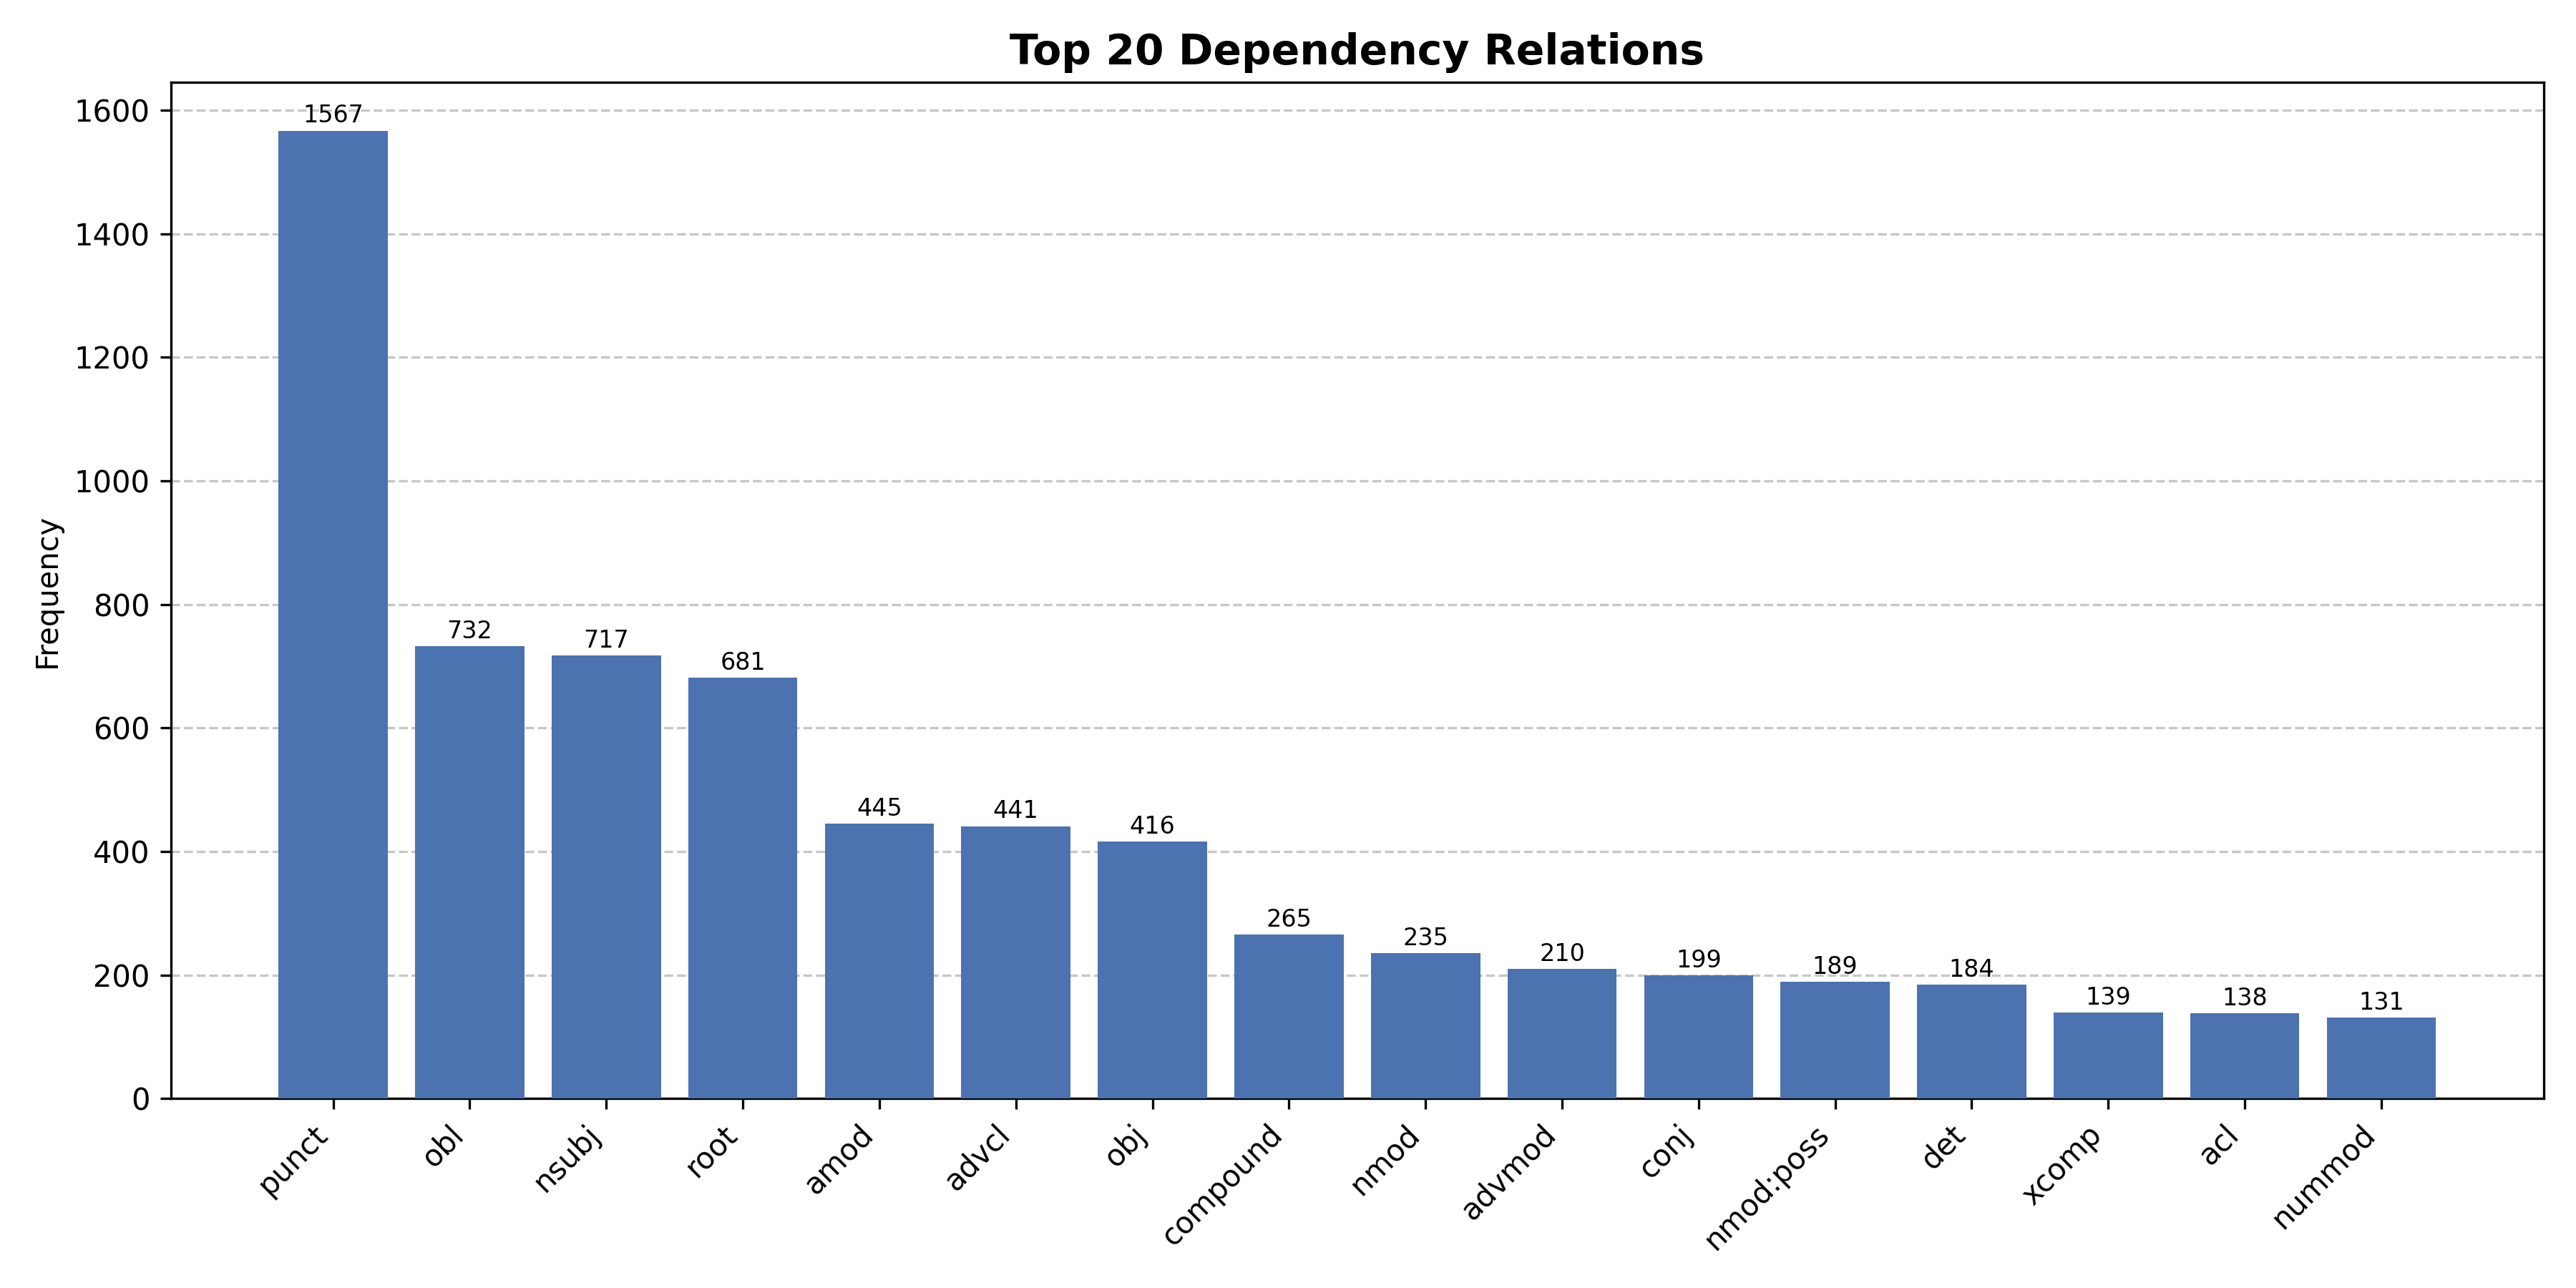
\includegraphics[width=\columnwidth]{Figure2_DepRel_Frequency.png}\\
      {\scriptsize Top-20 relation frequencies (combined corpus).}
    \column{.5\textwidth}
      \begin{table}
        {\scriptsize\setlength{\tabcolsep}{4pt}
        \begin{tabular}{lccc}
          \textbf{Relation} & \textbf{P} & \textbf{R} & \textbf{F1}\\
          \toprule
          \texttt{nummod}       & 75.0 & 86.5 & \best{80.4}\\
          \texttt{root}         & 72.9 & 74.5 & 73.7\\
          \texttt{case}         & 84.4 & 58.1 & 68.8\\
          \texttt{obj}          & 58.6 & 65.1 & 61.7\\
          \texttt{nsubj}        & 47.0 & 47.3 & 47.2\\
          \texttt{obl}          & 47.6 & 46.7 & 47.1\\
          \texttt{compound:lvc} & 36.7 & 54.6 & 43.9\\
          \texttt{nmod}         & 27.0 & 34.2 & 30.2\\
          \texttt{conj}         & 25.8 & 14.9 & \alert{18.9}\\
          \bottomrule
        \end{tabular}}
        \caption{spaCy S1.2 per-relation LAS F1 (\%).}
      \end{table}
  \end{columns}
\end{frame}

%% ---- Slide 13: Qualitative examples ------------------------
\begin{frame}{Qualitative parses from Stanza E2.2}%
             {Success vs a systematic light-verb failure}
  \begin{columns}[onlytextwidth, T]
    \column{.58\textwidth}
      \begin{block}{\small Success --- UAS = LAS = 100\%}
        \centering\vspace{2pt}
        \resizebox{\columnwidth}{!}{%
        \begin{dependency}[theme=simple]
          \begin{deptext}[column sep=0.28cm]
            bu \& bo'lim- \& asarlar \& bizga \& bu \&
            xazina- \& eshigini \& ochib \& beradi \& . \\
            \small pron \& \small adj \& \small noun \& \small pron
            \& \small pron \& \small noun \& \small noun
            \& \small verb \& \small verb \& \small pct \\
          \end{deptext}
          \depedge{2}{1}{det}
          \depedge{3}{2}{amod}
          \depedge{9}{3}{nsubj}
          \depedge{9}{4}{obl}
          \depedge{6}{5}{det}
          \depedge{7}{6}{nmod:poss}
          \depedge{8}{7}{obj}
          \depedge{9}{8}{xcomp}
          \deproot{9}{root}
          \depedge{9}{10}{punct}
        \end{dependency}}
        \vspace{2pt}
      \end{block}
    \column{.42\textwidth}
      \begin{block}{\small Failure --- \texttt{compound:lvc}}
        \centering\vspace{2pt}
        \resizebox{0.92\columnwidth}{!}{%
        \begin{dependency}[theme=simple]
          \begin{deptext}[column sep=0.42cm]
            bolalar \& o'yinni \& davom \& etdi \& . \\
            \small noun \& \small noun \& \small noun
            \& \small verb \& \small pct \\
          \end{deptext}
          \depedge{4}{1}{nsubj}
          \depedge{4}{2}{obj}
          \depedge[edge style={blue,thick}]{4}{3}{compound:lvc}
          \deproot{4}{root}
          \depedge{4}{5}{punct}
          \depedge[edge below,edge style={red,dashed}]{3}{1}{nsubj*}
          \depedge[edge below,edge style={red,dashed}]{3}{2}{obj*}
          \depedge[edge below,edge style={red,dashed}]{4}{3}{obj*}
        \end{dependency}}
        \vspace{2pt}
      \end{block}
      \vspace{4pt}
      {\scriptsize Gold (blue) vs predicted errors (red dashed).}
  \end{columns}
\end{frame}

%% ==============================================================
\section{Conclusion}
%% ==============================================================

%% ---- Slide 14: Conclusion ----------------------------------
\begin{frame}{Conclusion}{Practical guidance for Uzbek NLP pipelines}
  \begin{itemize}
    \item \alert{Pronounced trade-off}: transition-based tags better
          (+4.10 UPOS); graph-based parses far better
          (\best{+16.70 LAS}).
    \item \alert{Cross-treebank augmentation} is the single most
          impactful lever --- graph-based parsers exploit it best
          (\best{+9.62} vs +1.76 LAS).
    \item \alert{Recommendation}: graph-based parser + monolingual BERT
          + last-subword fusion when parsing accuracy is the goal.
  \end{itemize}
  \bigskip
  \footnotesize
  \textbf{Future work:} multi-seed testing; broader frameworks
  (UDPipe~2.0, Trankit, MaChAmp) and encoders (UzbBERT, XLM-R);
  LLM-based augmentation; parser ensembling.
\end{frame}

%% ---- Slide 15: Thank you (dark background) -----------------
{
\setbeamercolor{background canvas}{bg=edmdark}
\setbeamercolor{normal text}{fg=white}
\begin{frame}[plain]
  \edmlogo
  \vfill
  \begin{center}
    {\large\bfseries\color{white}
      Graph-Based vs Transition-Based\par
      Dependency Parsing for Uzbek\par}
    \vspace{1em}
    {\color{edmlight}
      Sanatbek Matlatipov \quad Maftuna Ismoilova \quad Mersaid Aripov\par}
    \vspace{0.5em}
    {\color{edmlight}\texttt{s.matlatipov@nuu.uz}\par}
    \vspace{1em}
    {\footnotesize\color{edmlight}
      Models: \texttt{huggingface.co/Sanatbek/uzudt}\par
      Code: \texttt{github.com/SanatbekMatlatipov/robust-parsing-uzbek}\par}
  \end{center}
  \vfill
  \begin{center}
    {\large\bfseries\color{white}Questions welcome.}
  \end{center}
\end{frame}
}

\end{document}
